\documentclass[dvips,11pt]{article}

% Any percent sign marks a comment to the end of the line

% Every latex document starts with a documentclass declaration like this
% The option dvips allows for graphics, 12pt is the font size, and article
%   is the style

\usepackage[letterpaper, margin=1in]{geometry}

\usepackage[pdftex]{graphicx}
\usepackage{url}
\usepackage[pdftex]{xcolor}
\usepackage{amsmath}
\usepackage{enumitem}
\usepackage{tabularx}

\usepackage{fancyhdr}
\pagestyle{fancy}
\fancyhf{}
\lfoot{2016 CFA Narrative 10565}
\rfoot{Page \thepage\ of \pageref{LastPage}}

\renewcommand{\headrulewidth}{0pt}
\renewcommand{\footrulewidth}{0.5pt}

\newcommand{\unc}[1]
{ \delta #1 }

\newcommand{\uncsq}[1]
{ \left(\unc{#1}\right)^2 }

\newcommand{\uncratio}[1]
{ \left(\frac{\unc{#1}}{#1}\right) }

\newcommand{\uncratiosq}[1]
{ \uncratio{#1}^2 }

\newcommand{\uncvector}[1]
{ \left[ \begin{array}{c} #1 \\ \delta #1 \end{array} \right] }

\newcommand{\comment}[1]
{{\bfseries \color{red} #1}}

\makeatletter
\renewcommand\section{\@startsection {section}{1}{\z@}%
                                   {-2.0ex \@plus -1ex \@minus -.2ex}%
                                   {2.3ex \@plus.2ex}%
                                   {\normalfont\bfseries}}% from \Large
\renewcommand\subsection{\@startsection{subsection}{2}{\z@}%
                                     {-2.0ex\@plus -1ex \@minus -.2ex}%
                                     {1.5ex \@plus .2ex}%
                                     {\normalfont\bfseries}}% from \large
\renewcommand\subsubsection{\@startsection{subsubsection}{3}{\z@}%
                                     {-2.0ex\@plus -1ex \@minus -.2ex}%
                                     {1.5ex \@plus .2ex}%
                                     {\normalfont\bfseries}}% from \normalsize
\makeatother


%----------------------------------------------------------------------------------------
%	DOCUMENT INFORMATION
%----------------------------------------------------------------------------------------
\begin{document}
\begin{centering}
  Application Narrative for DE-FOA-0001281\\
  \textbf{\large Error and Uncertainty Propagation for Fuel Cycle Calculations}\\
  2016 CFA Narrative 10565\\
\end{centering}
\vspace{1em}

\noindent\textbf{Technical Workscope Identifier:} FC-5.1b \hspace{1.5in} \textbf{Time Frame:} 3 years

\section{Introduction \& Proposed Scope}
Nuclear fuel cycle simulation tools can have a large
scope of application, from the study of the
behavior of a particular type of fuel or reactor inside an
existing nuclear fleet to the prospective analysis
of a complete nuclear transition. 
Each use case
requires a specific level
of confidence, which are up to now very
poorly assessed, if assessed at all.
Indeed, the only existing way to develop confidence in
any fuel cycle calculation/tool, is to compare
with other similar tools or historical
data.  For the former, the conclusion if often 
a list of why the different software gave
different results with no conclusion on the
precision of any.  The latter only allows
validation of existing concepts and has no impact
on calculations based on the use of new
concepts.

The aim of this project is to add error
propagation capability to the Cyclus fuel cycle
simulator\cite{Cyclus_paper}. Given the use case of predicting the
evolution of a large industrial enterprise in an
uncertain future, nuclear fuel cycle simulations
are generally based on approximate models and
uncertain input data.  Since strict validation is largely
considered to be impractical, such simulations are
seen as indications of trends in future behavior rather than
predictions of that behavior. Nevertheless, it
would be valuable to be able to place some
confidence bounds on those indications, both to
assess the robustness of conclusions that derive
from those indications and to provide information
about the sensitivity of those conclusions to the
uncertain data and algorithms.  Having a broad
distribution for each metric calculated in a fuel
cycle simulation instead of unique values will
allow a better comparison between different fuel
cycle scenarios.  Moreover for some critical
use cases, it could be extremely valuable to add
some degree of confidence on the results of the simulation.
This could result in confidence in the use of the tool for
such uses, and confidence in the conclusions that follow
from those results.

This project
will extend the Cyclus concept of resources to
include error information and then develop a
number of archetypes that can perform operations
to propagate that error in a manner that is 
consistent with the physical models of the 
archetype.
The ultimate calculation of fuel cycle performance
metrics will also need to be updated in order to
represent final results as distributions rather
than single values.  The primary outcome will
a demonstration of, and a
framework for, performing error propagation,
but not a comprehensive implementation of error
propagation for all models across all archetypes.
Other researchers will then be able to extend
this capability for additional archetypes, 
whether pre-existing or newly developed.

\section{Logical Path to Work Accomplishment}
The goal of this project is to add optional
extensions to Cyclus that will allow an assessment
of the error as it propagates through a fuel
cycle.  Four tasks are identified to accomplish
this goal.


\subsection{Task 1: Add uncertainty to resources}

The primary manifestation of uncertainty in a fuel
cycle simulation is in the composition of material
objects flowing through the system.  Thus the
primary task is to extend the standard Cyclus
material objects to inherently support an
uncertainty in their composition.  Each Cyclus
material is composed of both a total mass and a
vector representing the relative abundance of the
nuclides that make up that material.  While the
total mass of a material object may be subject to
some uncertainty, the composition vector is a more
interesting case.

Since these relative abundances are normalized,
the sum of a composition vector must be equal to
exactly one. Therefore, the uncertainty in the sum
must be equal to zero, the uncertainty in any one
nuclide is not independent of the uncertainty in
other nuclides.  If the mass\footnote{Cyclus 
is able to automatically and consistently switch
between mass, $\vec{m}$, and atom, $\vec{N}$, based
 definitions of a
material, and the discussion here will use 
whichever is convenient for the model being 
described.}
 of each nuclide, $i$,
is $m_i$, and its relative abundance is $f_i$,
then:
\begin{align*}
  \sum_i m_i = m_{tot} \qquad\qquad&\qquad\qquad  
       \sum_i \uncsq{m_i} = \uncsq{m_{tot}}\\
  f_i = \frac{m_i}{m_{tot}} \qquad\qquad&\qquad\qquad  
       \uncratiosq{f_i} = \uncratiosq{m_i} + \uncratiosq{m_{tot}}
\end{align*}

The data structures of a material object will be
extended to track the uncertainty in the
individual fractional abundances subject to these
relationships.

Cyclus provides a fixed set of operators for
creating and modifying material objects, largely
to ensure conservation of mass.  Most notably,
those operators include a method to divide a
material object into two and a method to combine
two material objects into one.  These operators
will each be modified to implement an algorithm
for error propagation that is appropriate to that
operator and subject to the above relationships.

When considering a material that is leaving any
given facility, there are three different sources
of uncertainty or error:
\begin{itemize}[nosep]
\item the isotopic inventory vector of the input,
  $\vec{m}_{in} = m_{tot,in} \cdot \vec{f}_{in}$,
  has an associated uncertainty $\unc{\vec{m}_{in}}$,
\item the uncertainty of parameters that define
that facility, $\unc{\tau_p}$, which correspond to
the possible  variation, or engineering tolerance,
in any physics parameter, $\tau_p$,
\item the modeling error, $\unc{{\cal M}}$,
introduced by the choice of approximate archetypes
models.
\end{itemize}
The uncertainty of the output material composition
is a function of all those uncertainties:
\begin{align}
  \delta \vec{m}_{out} = 
         {\cal F}\{~\unc{\vec{m}_{in}}~,~\unc{\vec{\tau}}~,~\unc{{\cal M}}~\}.
\end{align}

In this work we propose to introduce archetypes
that are able to combine all those sources and
compute the resulting uncertainties on the output
materials.  The following sections indicate which
specific archetypes will be considered with some
indication of the uncertain parameters that define
those archetypes.  In some cases, these archetypes
are modifications of those that are already part
of the Cycamore set of base archetypes.  In other
cases, entirely new models will be introduced to
enable more advanced uncertainty propagation.

Since many important fuel cycle metrics, such as
decay heat and radiotoxicity, are derived from the
flow and composition of the resource objects,
those metrics will need to be updated to be aware
of the error/uncertainty estimates, propagating
them into the metric evaluation and representing
them in a useful way to users.  For the most part,
this will require similar operations as are
necessary for the propagation of the errors within
the simulation.  However, visual representation of
the final metric results may require additional
development.

\subsection{Task 2: Update Cycamore archetypes for simple uncertainty propagation}

A set of standard archetypes are implemented and
distributed as part of the Cycamore package.
These archetypes use the simplest possible models
to approximate each of the facilities that they
represent.  In most cases, these models are too
simple to be the basis for a rigorous uncertainty
propagation model.  They are based heavily on user
input to approximate the physics and error
propagation may also require additional user
input.  All Cycamore archetypes will be assessed
for their role in error propagation in a full fuel
cycle simulation, with a minimum requirement that
output material uncertainty be at least as high as
input material uncertainty.  This can be
accomplished, to a large degree, through the
correct implementation of the material object
operators referred to in the previous section.
Although further analysis will be necessary to
confirm it, this simple approach is most likely
appropriate for the source, sink
and storage facilities.

\subsubsection{Cycamore separations facility}

Some facilities require additional considerations.
The Cycamore separations facility uses a simple
separation matrix approach to distribute every
nuclide, $i$, in the input material across $K$
different streams in the output.
\begin{equation}
N_{i,k} = N_{i,in} \cdot e_{i,k}
\end{equation}

The only parameter which can introduce extra
variance is the separation parameter for nuclide
$i$ in output stream $k$, $e_{i,k} \pm \delta
e_{i,k}$.  For this definition of the separation
parameter, $\sum_k e_{i,k} = 1$

Assuming that the uncertainty of the input
material and the tolerance of the separation
parameters are independent, the resulting
uncertainty on the output material composition can
express as:
\begin{align}
  \uncratiosq{N_{i,k}} = \uncratiosq{N_{i,in}} +  \uncratiosq{e_{i,k}}
\end{align}

In the limit of no uncertainty in the separation
parameters, this separated materials can be
generated purely by the material operators
described in the previous section.  How to
incorporate the additional source of uncertainty,
and its impact on the uncertainty of the total
mass will be addressed in this task.

\subsubsection{Cycamore enrichment facility}

The existing Cycamore enrichment facility produces
enriched uranium on demand, matching the
enrichment of each request, $k$.  Standard models
for enrichment flow rates and separative work
requirements are used only to determine the total
throughput of the facility in any time step as a
function of the:
\begin{itemize}[nosep]
\item inventory, $F_{tot}$, and composition,
  $x_f$, of feed material,
\item assay of the tails stream, $x_w$, and
\item total separative work, $S_{tot}$.
\end{itemize}
\begin{align*}
  \sum_k{F_k} \leq F_{tot}\qquad\qquad
  &\sum_k{S_k} \leq S_{tot}\\
  F_k = \frac{x_k - x_w}{x_f - x_w} P_k\qquad\qquad\qquad
  &W_k = \frac{x_k - x_f}{x_f - x_w} P_k\\
  S_k =  P_k\left(2x_k-1\right)ln\frac{x_k}{1-x_k}
         +W_k\left(2x_w-1\right)&ln\frac{x_w}{1-x_w}  
         -F_k\left(2x_f-1\right)ln\frac{x_f}{1-x_f}
\end{align*}

With this model, the uncertainty in the product
material is not determined by the inputs or the
model itself.  Instead, the uncertainty in product
enrichment can be introduced with a user-defined
tolerance parameter.  However, uncertainty in
the product enrichment can lead to uncertainty in
the amount of feed that is consumed by any request
and uncertainty in the amount of separative work
capacity that is consumed in order to fulfill each
request.  A user-specified tolerance on the tails
assay can also be introduced to contribute to
these uncertainties.  The uncertainty in these 
quantities can be determined using standard
formulas for propagation of error in analytic
expressions, and are omitted here for the sake of 
brevity.

The enrichment facility contributes constraints to
the network flow problem solved by the Cyclus
dynamic resource exchange (DRE) based on the
inventory of feedstock and the available
separative work.  Since such constraints define
the feasible solution space, uncertainty in these
parameters can have an impact on the operation of
the DRE.  Further analysis will be necessary to
upgrade the DRE to accommodate such uncertainty.

The Cycamore fuel fabrication facility will
probably involve a similar level of complexity as
it combines streams of material to approximate a
desired reactivity.

\subsubsection{Cycamore reactor facility}

The reactor archetype included in Cycamore is
based on fixed matched pairs of recipes for input
and output materials that are provided by the
user, in addition to all the classical reactor
parameters (batch number, cycle length, power,
capacity factor,...).  Such a model does not allow
any meaningful way to propagate uncertainty from
any input quantities into the output composition,
and simply requiring the user to provide uncertainty 
estimates on the output composition does not allow
any responsiveness to variations in the input
composition or its uncertainty.
Instead, the user will need to provide estimates
of the sensitivity of the output recipe's uncertainty to
variations in the input recipe's uncertainty.  In
general, each output isotope will be sensitive to
the uncertainty in every input isotope, although
in practice some of these can be ignored.
\begin{align}
\unc{N_{j,out}} = \sum_i \unc{N_{i,in}} \sigma_{i,j},
\end{align}
where $\sigma_{i,j}$ describes the relationship
between the uncertainty in output isotope $j$ and
uncertainty in input isotope $i$.  Since the
recipe reactor assumes a fixed input composition,
even if it does \textit{not} assume a fixed uncertainty in
that composition, these sensitivity parameters can
be written to depend only on the uncertainty of
the input composition and not on the composition
itself.  

This project will include a demonstration of one
way to estimate these sensitivities using a brute
force approach.  For any given input composition,
a full depletion calculation can performed to
arrive at an output composition.  Multiple
realizations of the input composition can be
sampled from a particular uncertainty of the input
composition to yield a population of output
compositions, from which an output uncertainty can
be measured.  If this is repeated for different
values of the input uncertainty, an approximation
of the sensitivity parameters can be performed.
The degree of approximation is consistent with
already crude approximation of the transmutation
model in the recipe reactor itself.

The Cycamore recipe reactor has many configuration
parameters that may also be uncertain.  One
example is the cycle length, typically expressed
in months.  A variation in the cycle length would
manifest itself as a variation in the burnup of
the fuel, and a similar approach to the one
described above can be used to estimate the effect
on the discharge inventory of the fuel.  A more
complete analysis of the set of parameters,
$\vec{\tau}$, will be performed as part of this work.

\subsection{Task 3: Introduce new archetypes for advanced uncertainty propagation}

Although the basis of many fuel cycle simulators,
the recipe reactor concept is overly rigid,
unresponsive to fluctuations that may arise in fuel
compositions, particularly in the presence of
recycling.  Similarly, the simple sensitivity
approach for propagating uncertainty in the recipe
reactor is very rigid and may not respond fully to
the uncertainties that may emerge.  The next level
of sophistication relies on interpolation on a set
of precomputed results from details depletion
calculations.  In addition to a number of ongoing
efforts to introduce a variety of interpolation
approaches to Cyclus\cite{brightlite, cyborg}, the
CLASS project\cite{CLASS} has developed a
stand-alone approach based on neural networks\cite{Leniau.ANE.2015}. The
CLASS methodology will be incorporated into Cyclus
modules and extended to include uncertainty
propagation.

\subsubsection{CLASS-based reactor facility} \label{sec:reactors}

A new reactor archetype will be introduced using
pre-trained models, ${\cal M}$, to predict key
physics parameters needed to compute the evolution
of a fuel during the irradiation. It has been
demonstrated that pre-trained neural network
models can be used to predict the evolution of the
one group cross sections of each nuclide (for
fission, capture and $n,2n$ reactions) during the
irradiation of the fuel from its initial isotopic
composition for a range of reactor concepts, from
LWR to SFR\cite{Leniau.ANE.2015, Leniau.PHYSOR.2016}.
These time-dependent cross sections are then used
by an ODE solver to determine the composition upon
discharge of the fuel.  For a neural network
predictor, ${\cal P}$, and an ODE solver, ${\cal S}$,
\begin{align}
  \vec{\Sigma}(t) &= {\cal P}^{\Sigma}\left( \vec{m}_{in}\right)\\
  \vec{m}_{out} &= {\cal S}\left( \vec{\Sigma}(t), \vec{m}_{in}\right)
\end{align}
Two approaches will be considered for extending
this neural network concept to uncertainty
propagation.

The first approach will develop an operator, 
${\cal K}$, to
estimate the errors in the cross-sections as 
a function of the initial composition:
\begin{align}
  \delta\vec{\Sigma}(t)  = {\cal K}\left( \vec{m}_{in}\right)  \equiv  \unc{{\cal P}^\Sigma\left( \vec{m}_{in}\right)} \label{eq:NNSigmaError}
\end{align}
and extend the ODE solver to combine the
uncertainty in the initial composition with the
error in the cross sections to estimate the
uncertainty in the final composition:
\begin{align}
  \uncvector{\vec{m}_{out}} = {\cal S^\prime}\left( \uncvector{\vec{\Sigma}(t)}, \uncvector{\vec{m}_{in}}\right)
\end{align}

The primary approach to approximating the error in
predicted cross sections will be to directly
compare the predicted cross section evolutions
with directly calculated cross section evolutions
for a variety of initial material compositions that
are not included in the set of data used to train
the neural networks.  Theoretically, the training
data itself is subject to uncertainty from its own
calculation methodology, but this source of
uncertainty will not be considered in this
project.

Uncertainty may also be introduced in the
user-defined model parameters, $\vec{\tau}$, but the
mechanism for doing so will depend on how each
parameter interacts with the physics model being
implemented.  The neural network model itself may
be able to provide insight on the uncertainty in
output composition caused by some model
parameters, \textit{e.g.} he burnup of the fuel at
discharge.

The second approach will attempt to use a new
neural network predictor, ${\cal P}^{\vec{m}}$, to
directly predict the fuel composition evolution:
\begin{align} \vec{m}_{out} = {\cal P}^{\vec{m}}\left( \vec{m}_{in}\right)
\end{align}
It is also necessary to estimate the error due to
the neural network prediction:
\begin{align}
  \left(\unc{\vec{m}_{out}}\right)_{\cal P}^{\vec{m}}= {\cal K}_1^{{\vec{m}}}(\vec{m}_{in})  \equiv \unc{{\cal P}^{\vec{m}}\left( \vec{m}_{in}\right)} \label{eq:NNModError}
\end{align}
and the propagation of the initial uncertainty:
\begin{align}
  \left(\unc{\vec{m}_{out}}\right)_{\unc{\vec{m}_{in}}} = {\cal K}^{{\vec{m}}}_2(\vec{m}_{in}, \unc{\vec{m}_{in}})
\end{align}

The operator to estimate the uncertainty due to
the neural network prediction, ${\cal
  K}_1^{{\vec{m}}}$, can be evaluated in the same way
as for operator ${\cal K}$ described in
Eq.\eqref{eq:NNSigmaError}. The operator to estimate
the propagation of the initial uncertainty,
${\cal K}_2^{{\vec{m}}}$ requires more investigation,
but could be implemented either as a neural
network itself, or with other techniques
(\textit{e.g.} kriging).

Once again, it is still necessary to consider the
mechanism for also incorporating uncertainty that
is introduced from variation in the parameters
that define the reactor's behavior.

\paragraph{Other errors:\\}

The sources of uncertainty considered above are
clearly not exhaustive. For example, as already
mentioned, the neural network will be trained on
simulated data which are subject to many different
errors/uncertainties (nuclear data uncertainty,
statistical error, modeling error...).  These
errors are outside the scope of this study.  The
aim of this project is to create a framework for
uncertainty/error propagation in fuel cycle
calculation and develop the require tool to do so.
Based on the success of this effort, other
projects may choose to tackle the other sources of
error and uncertainty.

\subsubsection{CLASS-based fuel fabrication} \label{sec:fabrication}

The aim of the fuel fabrication is to mix
different incoming material streams in order to
build a fuel composition that supports the
neutronics/physics requirement of the reactor. The
Cycamore fuel fabrication facility mixes two
streams of material using an equivalence method to
approximate a desired composition by matching its
initial reactivity.\cite{cycamore_fab}

By contrast, methods implemented in the CLASS
project have used a similar neural network
approach as described above to determine how to
mix multiple streams of material in order to
satisfy a number of reactor performance goals
including initial reactivity, burnup and/or
conversion ratio. As with the reactor models, the
predictive model is trained on the same set of
training depletion calculation used for the
reactor models. The capability of the neural
networks have been proven to predict the evolution
of the criticality in PWR reactor using MOX 
fuel\cite{Leniau.ANE.2015}, as well as
the the initial criticality of MOX fuel in 
SFR\cite{CLASS_UserGuide} and should be possible to
extend it to conversion ratio evolution.
\begin{align}
  \rho = {\cal P}^{\rho}\left( \vec{m}_{1},\vec{m}_{2}, \vec{\tau} \right)
\end{align}

Following the model described in \S
\ref{sec:reactors}, we will explore mechanisms to
estimate the error introduced by the neural
network prediction:
\begin{align}
  \left(\unc{\rho}\right)_{\cal P^\rho} = {\cal K}_1^{\rho}\left( \vec{m}_{1},\vec{m}_{2}, \vec{\tau} \right) \equiv \delta {\cal P}^\rho\left( \vec{m}_{1},\vec{m}_{2}, \vec{\tau} \right)
\end{align}
and separately, the propagation of the initial uncertainty and tolerance in the model parameters:
\begin{align}
  \left(\unc{\rho}\right)_{\unc{\vec{m}_{1}},\unc{\vec{m}_{2}},\unc{\vec{\tau}}} = {\cal K}^{\rho}_2\left( \uncvector{\vec{m}_{1}},\uncvector{\vec{m}_{2}}, \uncvector{\vec{\tau}} \right)
\end{align}

Initially, this model will be developed for MOX
fuel only, in LWR and SFR, used as both burners
and breeders.  The target parameters for the fuel
will depend on the type of reactor system, with
burnup being a typical LWR target parameter and
conversion ratio and initial reactivity used for
SFRs.

\subsection{Task 4: Demonstrate uncertainty propagation}

Verification and demonstration of the uncertainty
propagation will be performed in each stage of the
project, with a series of test cases that build
from the first task to the last.

Testing of the capabilities added in Task 1 will
include verification that the material
modification operators manage uncertainty in the
appropriate way and that the presence of
uncertainty information does not impact the
functioning of legacy archetypes that are unaware
of it.  It will also be necessary to test metrics
so that function correctly with and without the
presence of uncertainty.

Throughout tasks 2 and 3, as new archetypes are
enabled with the ability to track uncertainty, a
Total Monte Carlo approach will be used to measure
how well the uncertainty propagation has been
modeled.  Under this approach, a large number of
independent simulations will be performed, each
with a different randomly selected set of
parameters chosen from the uncertainty
distributions of the input quantities.  The
population of output quantities will be used to
measure the resulting uncertainty and compared
with the quantities calculated by the new
archetypes.  Each archetype will be tested on its
own before assembling larger problems.

With all the necessary components in place, a
series of demonstration simulations will be
conducted using fuel cycles of increasing
complexity: once through, MOX LWR recycle, and
fast reactor recycle.  These scenarios will be
constructed to highlight the role of error and
uncertainty and identify metrics in which the
presence uncertainty may impact fuel cycle
analysis conclusions.

\section{Relevance of Proposed Research}

This proposal aims to add an important and novel
feature to the field of fuel cycle simulation.
Since the precision of fuel cycle simulators has
never been assessed, this work might be a step
towards providing more confidence in the fuel
cycle simulation results.  While there have been
previous attempts to study uncertainty in isolated
cases\cite{visionEcon}, it has not been applied
across a full simulation

One outcome of this capability is the ability to
perform sensitivity studies that can indicate
which input parameters have the biggest impact on
the uncertainty of the output quantities of
interest.

Another outcome of this work will be the addition
of new responsive reactor and fuel fabrication
archetypes.  These archetypes will be based on
neural network capability already demonstrated by
other tools and will add to the suite of
archetypes available for general Cyclus use.

\section{Milestone Task Listing}

This research project consists of four major tasks
that will be conducted in parallel.  The first
task will extend over the first 9 months to
complete the basic implementation of uncertainty
in Cyclus materials and metrics.  Task 2 will
start simultaneously and extend for 20 months.
Task 3 represents the largest effort, beginning
after 6 months and continuing for 24 months.  Task
4 will begin with simple testing after 4 months
and continue for the duration of the project.

\begin{figure}[h!]
\centering
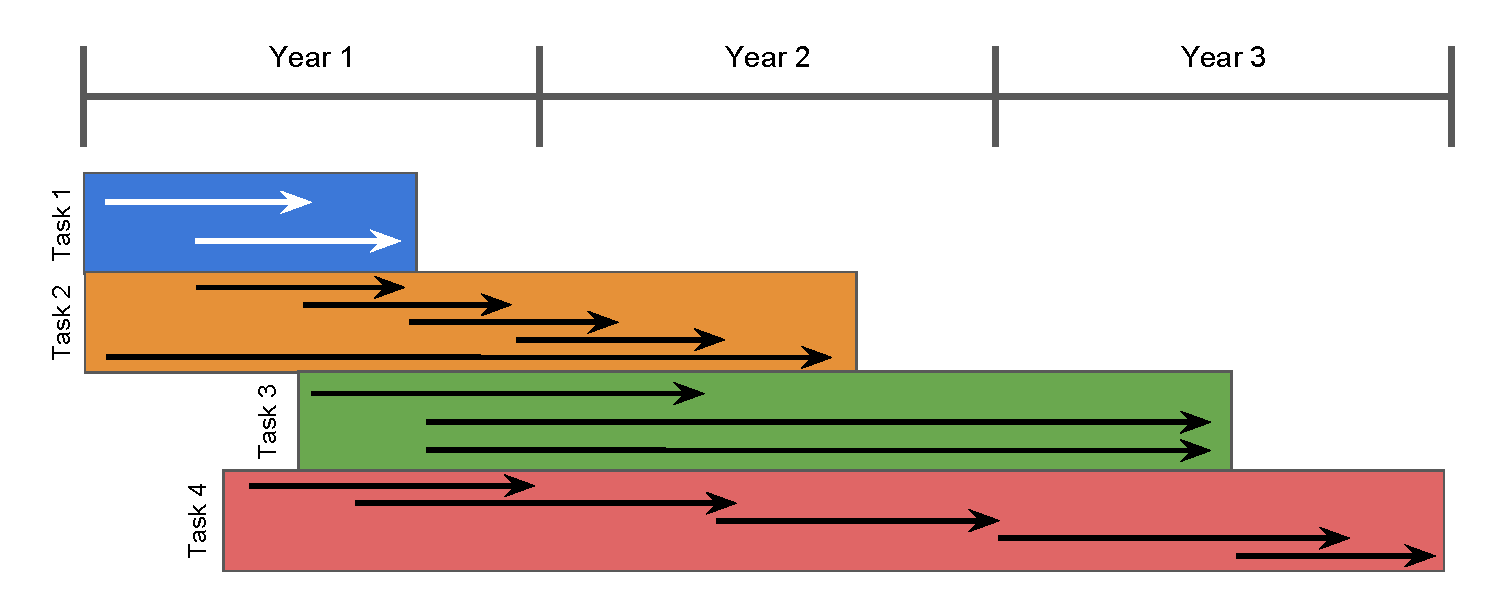
\includegraphics[width=\textwidth]	{timeline}
\caption{Preliminary schedule of the project indicating tasks and subtasks}
\label{fig:progression}
\end{figure}

\newpage
\noindent\textbf{TASK 1:} Cyclus update for uncertainty awareness
\begin{itemize}[nosep]
\item subtask 1: update material to uncertainty
\item subtask 2: update metrics to represent uncertainty
\end{itemize}

\noindent\textbf{TASK 2:} Updating Cycamore archetypes
\begin{itemize}[nosep]
\item subtask 1: source, sink and storage
\item subtask 2: enrichment facility 
\item subtask 3: separation facility
\item subtask 4: fuel fabrication facility
\item subtask 5: recipe reactor, including depletion calculations
\end{itemize}

\noindent\textbf{TASK 3:} Modeling development
\begin{itemize}[nosep]
\item subtask 1: isotopic space definition,
  training sample creation
\item subtask 2: reactor models development:
  parameter prediction, error analysis
\item subtask 3: fuel fabrication model
  development: parameter prediction, error
  analysis
\end{itemize}
 
\noindent\textbf{TASK 4:} Verification \& application
\begin{itemize}[nosep]
\item subtask 1: verification of basic material
  operations with uncertainty
\item subtask 2: demonstration of basic process
  with simplest archetypes calculation : source +
  enrichment + sink
\item subtask 3: demonstration of the overall
  process with extended Cycamore archetypes:
  enrichment + separation + recipe reactor
\item subtask 4: demonstration of modeling
  capabilities with new archetypes (Fab + reactor)
\item subtask 5: example calculation: PWR,
  transition from PWR to FBR
\end{itemize}

\begin{table}[h!]
\caption{List of major milestones and deliverables}
\begin{tabularx}{
\textwidth}{|X|c|l|}\hline
 \textbf{Milestone}       & 
     \textbf{Date}$^*$&
     \textbf{Deliverable} \\\hline
 Completion and testing of basic material operations      &   
     12                         & 
     Report on Tasks 1 \& 4.1   \\\hline
 Demonstration of uncertainty propagation with simple archetypes  &   
     18       & 
     Report on Tasks 2.1, 2.2 \& 4.2 \\\hline
 Demonstration of uncertainty propagation with extended Cycamore archetypes &
     24       &
     Report on Tasks 2.3, 2.4, 2.5 \& 4.3 \\\hline
 Demonstration of uncertainty propagation with CLASS-based archetypes &
     33       &
     Report on Tasks 3 \& 4.4 \\\hline
 Demonstration of uncertainty propagation on representative fuel cycle transitions &
     36       &
     Final report\\\hline
\end{tabularx}
{\footnotesize $^*$ all dates are given in months from project start}
\end{table}

\section{Facilities}

Most of the development work for this project will
be carried out on desktop workstation or laptop
computers with free and open source software
and software libraries. Desktop computing
capabilities are available to the investigators;
where additional computing platforms are required
(for instance, for graduate students working on
the project), funding for them is requested.

Where larger computational resources are required,
the lead institution maintains a variety of
centrally-supported computing resources, including
a large pool of distributed computing resources
and a growing tightly coupled high performance
computing resource. The distributed computing pool
gives researchers access to over 10,000 computing
cores, and seamless capability of reaching the
nationally distributed Open Science
Grid. Combined, these resources routinely provide
researchers with approximately 300,000 CPU hours
per day. If the algorithms favor a high
performance computing mode, the cluster at has
over 3000 cores with 30 TB of RAM, connected with
a 56 GB/s Infiniband backplane.

\section{Quality Assurance \& Software Development Process}

\textit{This project will comply with all Quality
  Assurance requirements, as described on the NEUP
  website.}  

This work will follow the Cyclus development
model.  We will employ a variety of modern
software project management tools: revision
control, automated testing, automated and manual
documentation, bug tracking. Related projects at
are already managed under source code revision
control system (git) that provides detailed
tracking of all changes to the code base. A test
suite has been developed and new tests will be
added for each new capability. This test suite
will be automatically executed with each proposed
change in the revision control system to identify
any flaws that may be introduced. Automated
documentation tools are used in the source code to
create a detailed reference for the interfaces and
additional background documentation. Out-of-code
detailed reports and publications will supplement
the information on each new capability. Finally, a
bug tracking system (GitHub issues) is deployed to
help users and developers to understand known
issues and to track their resolution as a
developer community. As new capability is added,
it will come under the same quality assurance
practices as described here for the existing
capabilities.

%----------------------------------------------------------------------------------------
%	BIBLIOGRAPHY
%----------------------------------------------------------------------------------------

\bibliographystyle{narrative}

\bibliography{narrative}

%----------------------------------------------------------------------------------------

\label{LastPage}
\end{document}
